\documentclass{beamer}
  % Beamer settings
  \usetheme{CambridgeUS}
  \usecolortheme{seagull}
  \usefonttheme{professionalfonts}
  \usefonttheme{serif}

  % Packages and package settings
  \usepackage{fontspec}
    \setmainfont{Charis SIL}
  \usepackage{hyperref}
    \hypersetup{colorlinks=true,
                allcolors=blue}
  \usepackage[backend=biber, style=apa]{biblatex}
    \addbibresource{References.bib}
  \usepackage{graphicx}
    \graphicspath{{./figures/}}
  \usepackage[french]{babel}

  % Document information
  \author{Joshua McNeill}
  \date{28 janvier 2020}
  \title{Exposé de Dewaele (1999)}

\begin{document}
  \begin{frame}
    \titlepage
  \end{frame}

  \begin{frame}{Article}
    \fullcitebib{dewaele_word_1999}
  \end{frame}

  \begin{frame}{Plan}
    \tableofcontents
  \end{frame}

  \AtBeginSection{
    \begin{frame}{Plan}
      \tableofcontents[currentsection]
    \end{frame}
  }

  \section{Introduction}
    \begin{frame}
      \begin{block}{Objectif}
        Comparer les interrogatives utilisées par les locuteurs natifs (LN) contre non-natifs (LNN)
      \end{block}
      \begin{block}{Question de recherche}
        «Les locuteurs avancés du français diffèrent-ils des LN dans leurs usages des structures interrogatives?»
        \begin{itemize}
          \item Si c'est le cas: Les LNN préfèrent-ils les structures plus formelles?
        \end{itemize}
      \end{block}
    \end{frame}

    \begin{frame}
      \begin{block}{Hypothèses}
        Il y aura une différence entre les LN et les LNN, et
        \begin{itemize}
          \item Les LNN préféreront les structures plus formelles
        \end{itemize}
        C'est ce que Dewaele (1992) a trouvé pour l'effacement du \emph{ne} parmi des étudiants flamands
      \end{block}
    \end{frame}

    \begin{frame}{Variables}
      \begin{block}{Deux formes générales}
        \begin{itemize}
          \item Interrogatives totales (IT): Cela cherche une décision
          \item Interrogatives partielles (IP): Cela cherche des informations
        \end{itemize}
      \end{block}
    \end{frame}

    \begin{frame}{Variables}
      \begin{block}{}
        Interrogatives totales
      \end{block}
      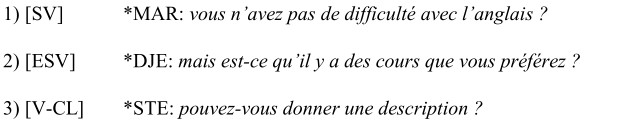
\includegraphics[scale=0.5]{interrogatives_totales.jpg}
      \begin{block}{}
        Interrogatives partielles
      \end{block}
      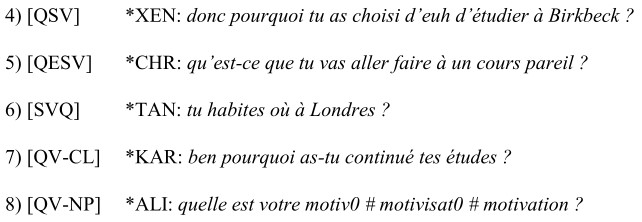
\includegraphics[scale=0.5]{interrogatives_partielles.jpg}
    \end{frame}

    \begin{frame}{Variabilité}
      \begin{block}{}
        Coveney (1996) a trouvé un éventail de variabilité dans 10 corpus
      \end{block}
      \begin{block}{Au Québec}
        Lightbrown (1980) et Lightbrown \& d'Anglejean (1985) ont trouvé une préférence pour les structures non-inverties
        \begin{itemize}
          \item Lyster (1996) a trouvé l'inverse
          \item Il a considéré des inversions les structures avec \emph{-ti}:
          \item «Je peux-ti t'aider?»
          \item (45 \emph{-ti}, 122 inverties, 129 non-inverties)
        \end{itemize}
      \end{block}
    \end{frame}

    \begin{frame}{Facteurs prescriptifs}
      \begin{block}{Une hiérarchie de formalité (Grevisse 1980; Wagner \& Pinchon 1962)}
        \begin{itemize}
          \item Style formel: [V-CL], [QV-CL], [QVGN] (l'inversion)
          \item Neutre mais inapproprié dans l'écriture: [ESV], [QESV] (\emph{est-ce que})
          \item Familier: [SV], [SVQ]
          \item Encore plus familier: [QSV]
        \end{itemize}
      \end{block}
      \begin{block}{Il y a des exceptions}
        «Pourquoi veux-tu qu'on parte?» n'est pas formel (Huot 1997)
      \end{block}
    \end{frame}

    \begin{frame}{Facteurs descriptifs}
      \begin{block}{Dans Coveney (1996)}
        \begin{itemize}
          \item Les IT: C'est des facteurs pragmatiques
          \item Les ESV: Quand on attend une réponse
          \item Les SVQ: Quand le sujet ou le verbe porte moins d'informations
          \item Les QSV: Ce sont les hommes qui les préfèrent plus que les femmes
        \end{itemize}
      \end{block}
      \begin{alertblock}{}
        Les interrogatives dans Coveney (1996) avaient plus de fonctions
      \end{alertblock}
    \end{frame}

  \section{Méthode}
    \begin{frame}{Participants}
      \begin{block}{}
        \begin{itemize}
          \item $N = 20$
          \item 5 LN, 15 LNN
          \item 9 femmes, 11 hommes
          \item âgés de 20 à 60 ans
        \end{itemize}
      \end{block}
      \begin{block}{}
        Tous étaient des étudiants du département de français à l'Université de Londres
      \end{block}
    \end{frame}

    \begin{frame}{Collecte de données}
      \begin{block}{Questionnaires pour obtenir des informations diastratiques}
        Genre, âge, temps passé en France, autres langues, profession, etc.
      \end{block}
      \begin{block}{Interviews}
        Regroupés en pairs
        \begin{itemize}
          \item Moitié les mêmes genres, moitié mixtes
          \item Deux séances d'une heure chacune
          \item Un participant a interviewé l'autre pendant 15 minutes avant d'inverser les rôles
        \end{itemize}
      \end{block}
      \begin{block}{}
        Corpus total: 25068 mots
      \end{block}
    \end{frame}

  \section{Résultats}
    \begin{frame}[t]{Comparaison avec des études antérieures}
      \begin{columns}
        \column{0.5\linewidth}
          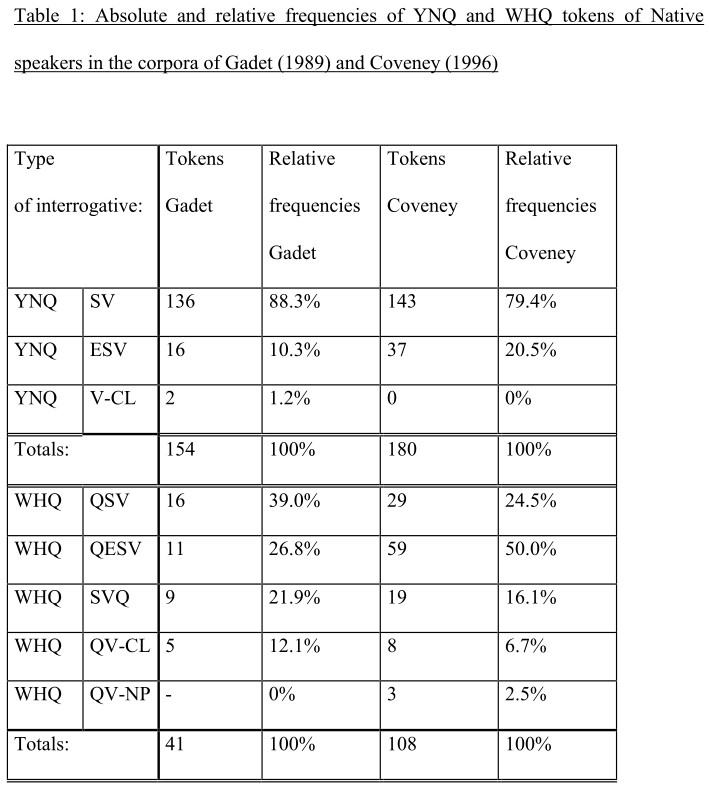
\includegraphics[scale=0.32]{gadet_coveney.jpg}
        \column{0.5\linewidth}
          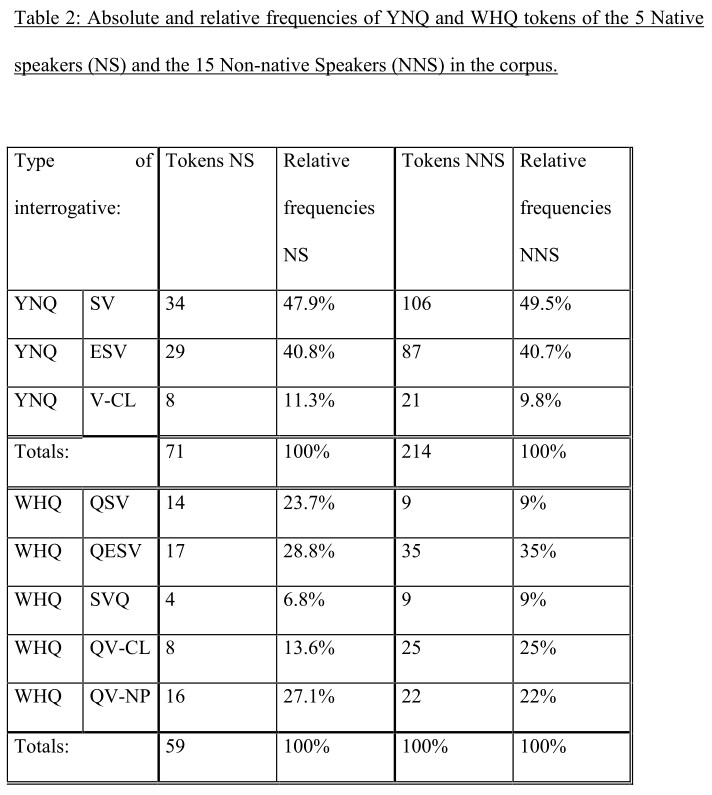
\includegraphics[scale=0.32]{resultats.jpg}
      \end{columns}
    \end{frame}

    \begin{frame}{Pourquoi plus d'inversion?}
      \begin{block}{Une différence de contexte}
        \begin{itemize}
          \item Coveney: À une colonie de vacances
          \item Gadet: Des amis au téléphone
          \item Dewaele: Dans une \emph{université}
        \end{itemize}
      \end{block}
    \end{frame}

    \begin{frame}[t]{Facteurs}
      \begin{columns}
        \column{0.5\linewidth}
          \begin{block}{Différences selon les variables diastratiques}
            Aucune signification pour:
            \begin{itemize}
              \item l'âge,
              \item le genre,
              \item l'histoire linguistique,
              \item la motivation et
              \item la première langue
            \end{itemize}
            Une signification:
            \begin{itemize}
              \item Locuteurs natifs contre non-natifs pour les interrogatives partielles
            \end{itemize}
          \end{block}
        \column{0.5\linewidth}
          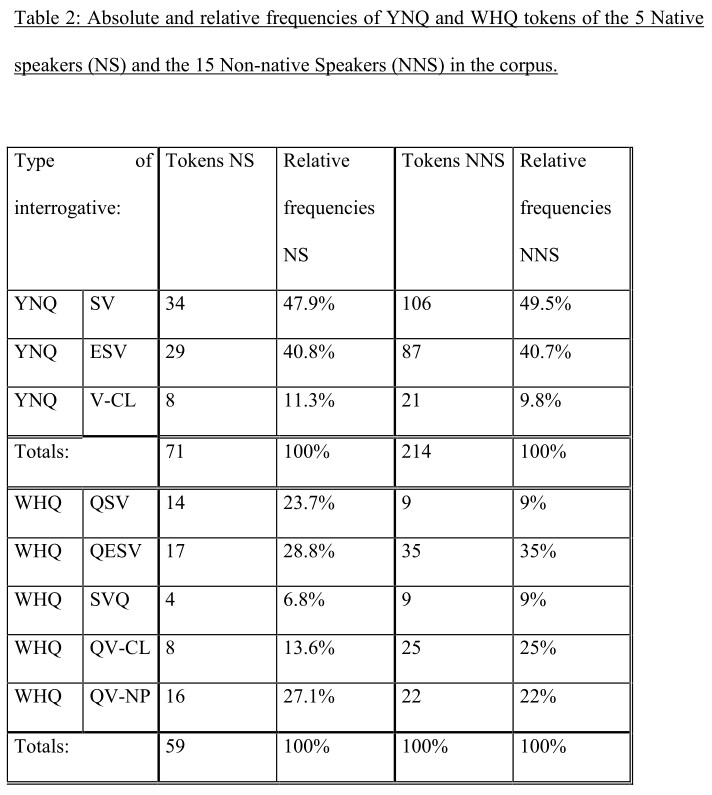
\includegraphics[scale=0.32]{resultats.jpg}
      \end{columns}
    \end{frame}

    \begin{frame}[t]{Facteurs verbaux et de temporels}
      \begin{columns}
        \column{0.47\linewidth}
          \begin{minipage}[t][0.6\textheight]{\linewidth}
            \begin{block}{}
              Différences selon les verbes\phantom{p}
            \end{block}
            \begin{tabular}{l r}
              \emph{Verbe} & \emph{Fréquence d'inversion} \\
              \hline
              avoir        & 23 \\
              pouvoir      & 7 \\
              trouver      & 6 \\
              faire        & 4 \\
              vouloir      & 3
            \end{tabular}
          \end{minipage}
        \column{0.53\linewidth}
          \begin{minipage}[t][0.6\textheight]{\linewidth}
            \begin{block}{}
              Différences selon les temps
            \end{block}
            \begin{tabular}{l r}
              \emph{Temps} & \emph{\% des interrogatives} \\
              \hline
              Présent      & 78,2 \\
              Passé        & 16,0 \\
              Conditionnel & \\
              ou futur     & 5,7
            \end{tabular}
          \end{minipage}
      \end{columns}
      \begin{block}{}
        Parmi les inversions clitiques: 84,2\% des structures étaient au présent
      \end{block}
    \end{frame}

    \begin{frame}{Facteurs pragmatiques}
      \begin{block}{}
        Presque toutes les inversions [V-CL] et [QV-CL] ont introduit de nouveaux sujets (95\%)
      \end{block}
      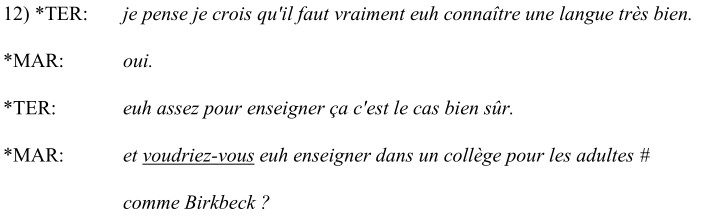
\includegraphics[scale=0.6]{inversion.jpg}
    \end{frame}

    \begin{frame}{Facteurs linguistiques}
      \begin{block}{}
        \begin{itemize}
          \item Les LNN évitent les [QSV] mais pas les [SV]
          \item Les LNN utilisent plus de [QV-CL]
        \end{itemize}
      \end{block}
      \begin{block}{Selon Dewaele, c'est une influence possible de l'anglais}
        \begin{itemize}
          \item L'anglais permet [SV] mais pas [QSV]
          \item {[}QV-CL] existe en anglais
        \end{itemize}
      \end{block}
    \end{frame}

  \section{Conclusion}
    \begin{frame}{Significations et remarques}
      \begin{block}{Pour les IP uniquement}
        Les LNN utilisent des variantes plus formelles que les LN
      \end{block}
      \begin{block}{}
        Les inversions étaient plus fréquentes que dans les études antérieures chez les LNN et les LN
      \end{block}
    \end{frame}
\end{document}
